\section{Introducci\'on}

En esta sección se implementarán heurísticas de búsqueda local para tratar de resolver el problema de $k-PMP$, intentando con diferentes métodos para alcanzar una solución y diferentes vecindades.

Para ello, partiendo de una solución generada al azar, se intentará a través de sucesivas iteraciones analizar cierta vecindad para intentar mejorar la solución existente y aproximarse más a una 'buena' solución en un tiempo aceptable. 

Por lo tanto debemos tener en cuenta de no hacer las vecindades ni muy grandes, ya que esto puede llevar a una pérdida de performance, ni muy pequeñas, ya que esto puede llevar a que el algoritmo explore sólo una pequeña cantidad de soluciones y devuelva una solución muy alejada del óptimo.

Como primera idea para una vecindad tomaremos cada nodo del grafo, vemos cuánto peso agrega en la suma intraconjunto en que se encuentra, lo quitaremos de este conjunto e intentamos meterlo en todos los demás, viendo si en alguno logra minimizar esta suma. En caso afirmativo, lo sacamos de su antiguo conjunto y lo ponemos en el nuevo. Realizamos esto hasta que deja de ser posible mejorar la solución y en este punto la devolvemos.


Otra vecindad que plantearemos será buscar el nodo que más peso está generando en la suma intrapartición, quitarlo de la partición donde se encuentra y agregarlo a alguna otra.

Finalmente se implementará una tercera busqueda local que quite dos nodos que están en una misma partición e intente buscar alguna otra donde los mismos sumen un menor peso intrapartición.

Los algoritmos escritos de manera formal serán así:

\begin{algorithm}
  	\begin{algorithmic}[1]\parskip=1mm
		 \caption{ Busqueda1(SoluciónInicial) }
		 	\STATE{Guardo SoluciónInicial en SolucionPrevia}
	 		\STATE{Mientras en el paso anterior se haya mejorado SolucionPrevia} 
				\STATE{\quad Para todo nodo $i$ de $1$ a $n$ del grafo ~~~~ $\mathcal{O}(n)$}
		 		\STATE{\quad Miro que peso agrega el nodo $i$ en el conjunto asignado por SolucionPrevia  $\mathcal{O}(n)$}
		 		\STATE{\quad Miro que peso agrega el nodo $i$ quitandolo del conjunto asignado y poniendolo en los demas $\mathcal{O}(n)$}
				\STATE{\quad \quad Si algun conjunto $M$ obtengo un peso menor, modifico SolucionPrevia $\mathcal{O}(n^2)$}
				\STATE{\quad \quad Asigno $i$ al conjunto $M$ $\mathcal{O}(1)$}   
				\STATE{\quad \quad Itero}
	\end{algorithmic}
\end{algorithm}

En el paso "Miro qué peso agrega el nodo $i$ quitándolo del conjunto asignado y poniéndolo en los demás", que dado que todo nodo puede estar sólo en un conjunto, iterando sobre todos los elementos de los conjuntos, al menos voy a iterar n veces, de ahí la complejidad $\mathcal{O}(n)$.

Dada nuestra implementación de conjunto con listas simplemente enlazadas, encontrar un elemento y borrarlo cuesta $\mathcal{O}(n^2)$ por esta razón modificar solución previa tendrá esta complejidad. Utilizando listas doblemente enlazadas esto se hubiera podido reducir a $\mathcal{O}(n)$ pero por falta de tiempo no se implementó.

\begin{algorithm}
  	\begin{algorithmic}[1]\parskip=1mm
		 \caption{ Busqueda2(SoluciónInicial) }
			\STATE{Guardo SoluciónInicial en SolucionPrevia}
	 		\STATE{Mientras en el paso anterior se haya mejorado SolucionPrevia}
			\STATE{Asigno $j = 1$}
				\STATE{\quad Tomo el j-esimo nodo mas pesado de la SolucionPrevia, al que llamo $i$ $\mathcal{O}(1)$}
		 		\STATE{\quad Miro que peso agrega el nodo $i$ en el conjunto asignado por SolucionPrevia $\mathcal{O}(n)$}
		 		\STATE{\quad Miro que peso agrega el nodo $i$ quitandolo del conjunto asignado y poniendolo en los demas $\mathcal{O}(n)$}
				\STATE{\quad \quad Si En algun conjunto $M$ obtengo un peso menor}   
				\STATE{\quad \quad \quad modifico SolucionPrevia y asigno $i$ al conjunto $M$ $\mathcal{O}(n^2)$}
				\STATE{\quad \quad \quad Itero}
				\STATE{\quad \quad Si no, sumo $1$ a $j$}
				\STATE{\quad \quad Si $j == n$}
				\STATE{\quad \quad \quad Devuelvo SolucionPrevia}
				\STATE{\quad \quad Si no}
				\STATE{\quad \quad \quad Itero}
	\end{algorithmic}
\end{algorithm}

\begin{algorithm}
  	\begin{algorithmic}[1]\parskip=1mm
		 \caption{ Busqueda3(SoluciónInicial) }
		 	\STATE{Guardo SoluciónInicial en SolucionPrevia}
	 		\STATE{Mientras en el paso anterior se haya mejorado SolucionPrevia} 
				\STATE{\quad Para todo nodo $i$ de $1$ a $n$ del grafo $\mathcal{O}(n)$}
				\STATE{\quad\quad Tomo otro nodo $k$ del mismo conjunto de $i$ $\mathcal{O}(1)$}
		 		\STATE{\quad\quad Miro que peso agrega el nodo $i$ y $k$ en el conjunto asignado por SolucionPrevia $\mathcal{O}(n)$}
		 		\STATE{\quad\quad Miro que peso agrega el nodo $i$ y $k$ quitandolo del conjunto asignado y poniendolo en los demas $\mathcal{O}(n)$}
				\STATE{\quad\quad \quad Si algun conjunto $M$ obtengo un peso menor, modifico SolucionPrevia $\mathcal{O}(n^2)$}
				\STATE{\quad\quad \quad Asigno $i$ y $k$ al conjunto $M$ $\mathcal{O}(1)$}   
				\STATE{\quad\quad \quad Itero}
	\end{algorithmic}
\end{algorithm}

\newpage

\section{Análisis de Complejidades}

Aquí analizaremos las complejidades de los diferentes algoritmos. Para cada uno de ellos elegimos una implementación con matriz de adyacencias para modelar el peso de las aristas y un vector de longitud variable para implementar los diferentes conjuntos.

Para el primero, cada paso de búsqueda local tendrá una complejidad de peor caso de $O(n(n + n + n^2))$. Ahora si $k$ es mayor a $n$ quiere decir que hay más subconjuntos disponibles que nodos, lo que llevaría a una solución trivial donde cada nodo va en un subconjunto diferente y la solución para $k-PMP$ sería 0.
Luego podemos acotar a $k$ por $n$ con lo que se obtendría una complejidad igual a $O(n^3)$

Para el segundo algoritmo, por cada iteración del algoritmo la complejidad será $O(n^2)$ para calcular el nodo con mayor peso del grafo. $O(n)$ para determinar si existe una mejor partición donde este nodo pueda estar y, en el caso de que exista, $O(n^2)$ para quitarlo de la partición anterior y agregarlo a la nueva. Luego, nuevamente acotando $k$ por $n$, se obtiene una complejidad para cada paso de la iteración de $O(n^2)$.

El tercer algoritmo es simplemente el primer algoritmo pero esta vez para cada nodo además tomo un vecino, y realizo el mismo procedimiento que antes, esto para cada vecino, suponiendo que en el peor caso, para un nodo todos los otros nodos esten en el mismo conjunto, se tendrá que realizar el procedimiento de antes la misma cantidad de veces solo que ahora para dos nodos distintos, luego la complejidad continúa siendo $O(n^2 (n + n k + n^2))$. Acotando nuevamente $k$, obtenemos que el algoritmo es: $O(n^3)$

\section{Testing}

En esta sección comprobaremos de manera empírica las complejidades antes calculadas y luego una comparación entre las tres diferentes heurísticas.

Para ello, al igual que para el algoritmo goloso, tomamos grafos completos con 25 a 100 nodos, y comparamos los diferentes tiempos obtenidos:

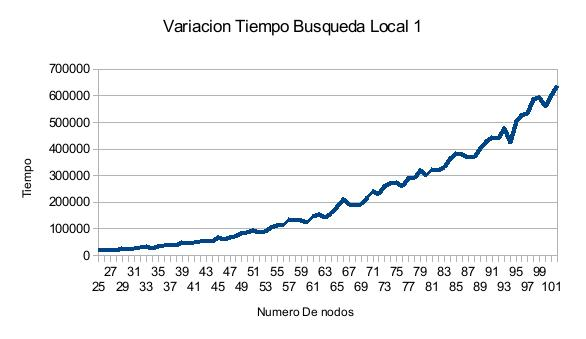
\includegraphics[scale=0.5]{Ej4/tiempo1.jpg}

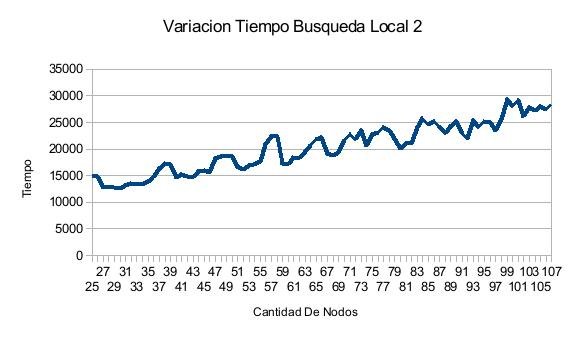
\includegraphics[scale=0.5]{Ej4/tiempo2.jpg}

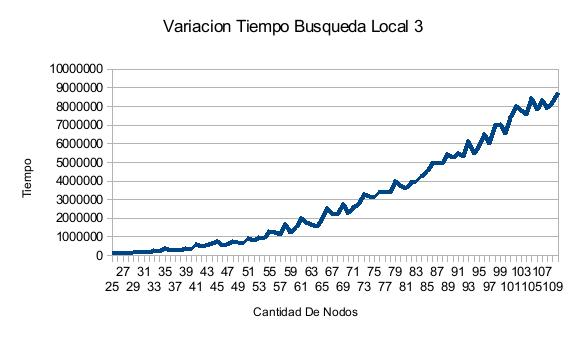
\includegraphics[scale=0.5]{Ej4/tiempo3.jpg}

Puede verse que si bien existe cierto ruido en la toma de muestras, causado muy posiblemente por el hecho de que para cada grafo, el número de veces que es posible continuar mejorando la solución sea variable y poco controlable. Existe una tendencia muy marcada en los tres algoritmos.

Para poner más en evidencia esto, dividiremos por las complejidades teóricas para así hacer más evidente este patrón:

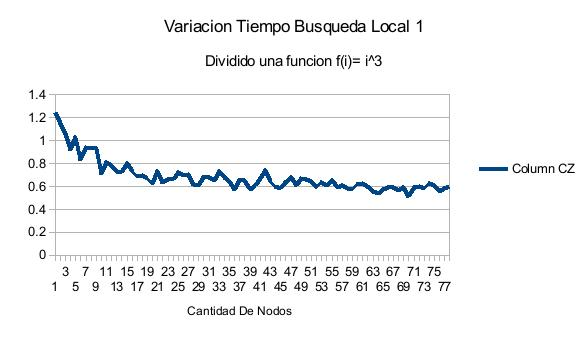
\includegraphics[scale=0.5]{Ej4/tiempo1div.jpg}

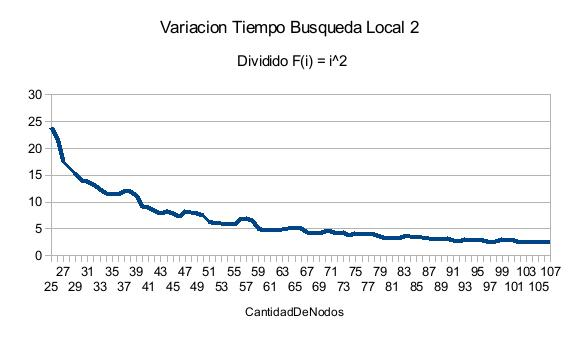
\includegraphics[scale=0.5]{Ej4/tiempo2div.jpg}

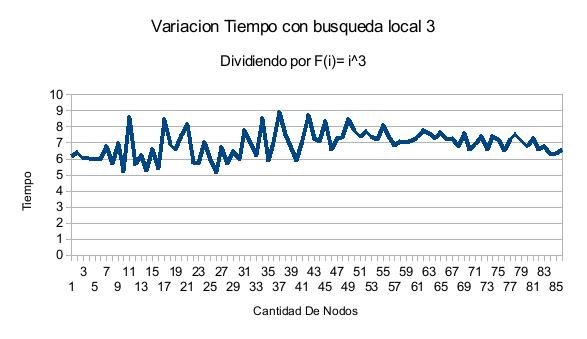
\includegraphics[scale=0.5]{Ej4/tiempo3div.jpg}

Como puede verse, en los tres casos las heurísticas están acotadas por las complejidades calculadas en el apartado anterior.

Veamos como se comportan las busquedas locales contra el algoritmo exactos para $K_23$ con peso en las aristas entre $1$ a $100$ elegidos de forma uniforme, tomaremos 100 muestras y compararemos los resultados contra el algoritmo de backtracking.

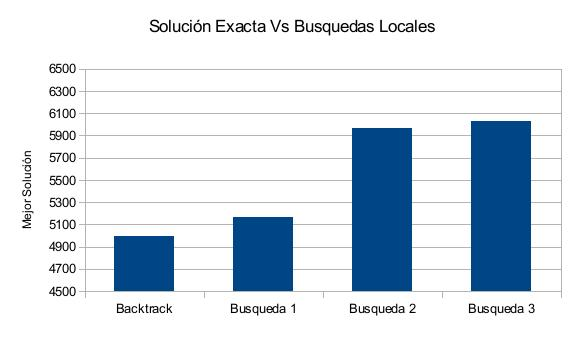
\includegraphics[scale=0.5]{Ej4/solucionestodos.jpg}

Puede verse que el que mejor aproxima a las soluciones reales es la primera búsqueda local. Y no solo eso, de los 100 casos tomados, la búsqueda local 1 logra encontrar la solución exacta a 13 de las instancias! mientras que las otras dos heurísticas en ninguno de los casos logran encontrar la solución exacta.

Además, para estas instancias se realiza a modo comparativo un promedio de los tiempos que tardan en encontrar la solución, esto es lo que se obtiene:

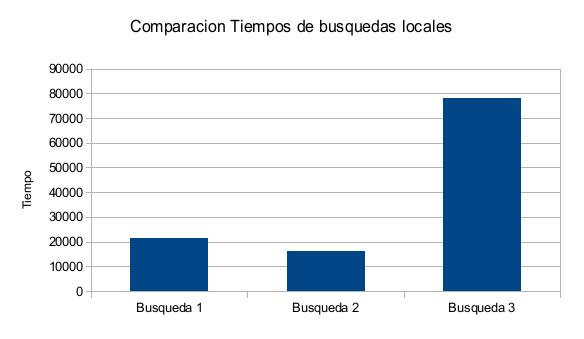
\includegraphics[scale=0.5]{Ej4/tiempotodos.jpg}

Por lo que en primera instancia, el algoritmo de búsqueda local 1 es bastantemente superior en todo sentido a los otros dos, ya que encuentra soluciones exactas y obtiene tiempos empíricos mucho mejores que los otros dos algoritmos.
